\documentclass[12pt,a4paper]{article}

\usepackage[in, plain]{fullpage}
\usepackage{array}
\usepackage{../../../moncours2}

\toggletrue{eleve}
%\toggletrue{dys}


\graphicspath{{./img/}}
\date{}
\title{\textcircled{{\normalsize{3}}} Nombres relatifs}

\renewcommand{\labelitemi}{∙}
%
%\rfoot{Page \thepage}
\begin{document}
	%
	%\dominitoc
	%
	%\tableofcontents
	
	\maketitle

\begin{myobj}
	\begin{itemize}
		
		\item Construire le symétrique d’un point ou d'une figure par rapport à une droite à la main où à l’aide d’un logiciel;
		\item Construire le symétrique d’un point ou d'une figure par rapport à un point, à la main où à l’aide d’un logiciel;
		\item Utiliser les propriétés de la symétrie axiale ou centrale;
		\item Identifier des symétries dans des figures.		
	\end{itemize}
\end{myobj}

\begin{mycomp}
	\begin{itemize}
		\item \kw{Chercher (Ch2)} :  s’engager    dans    une    démarche    scientifique, observer, questionner, manipuler, expérimenter (sur une feuille de papier, avec des objets, à l’aide de logiciels), émettre des hypothèses, chercher des exemples ou des contre-exemples, simplifier ou particulariser une situation, émettre une conjecture ;
		\item \kw{Raisonner (Ra3)} :  démontrer : utiliser un raisonnement logique et des règles établies (propriétés, théorèmes, formules) pour parvenir à une conclusion ;
		\item \kw{Communiquer (Co2)} :  expliquer à l’oral ou à l’écrit (sa démarche, son raisonnement, un calcul, un protocole   de   construction   géométrique, un algorithme), comprendre les explications d’un autre et argumenter dans l’échange ; 
		
	\end{itemize}
\end{mycomp}




\section{Définitions}

\begin{mydef}
	$a$ et $b$ sont deux nombres ($b$ $\neq$ 0).\pause Le \kw{quotient} de $a$ par $b$ se note $a \div b$ ou $\dfrac{a}{b}$, en écriture fractionnaire.\pause
\end{mydef}

\begin{myex}
	%\begin{itemize}
		%\item 
		Le quotient de 5 par 4 est $\dfrac{5}{4}$, c'est le nombre qui multiplié par 4 donne 5. \pause
		\begin{equation*}
			\dfrac{5}{4} \times 4 = 5
		\end{equation*}

		%\item Le quotient de 2 par 3 est $\dfrac{2}{3}$, c'est le nombre qui multiplié par 3 donne 2. $\dfrac{2}{3} \times 3 = 2 $.
	%\end{itemize}
\end{myex}

\begin{mydef}
	Si $a$ et $b$ sont entiers, alors $\dfrac{a}{b}$ est une \kw{fraction}.\pause $a$ est le\pause \kw{numérateur} et $b$ est le\pause \kw{dénominateur}.	
	
\end{mydef}

\begin{center}
	\includegraphics*[scale=0.5]{def}
\end{center}

\begin{myex}
	$\dfrac{\num{4.2}}{\num{2}}$, $\dfrac{\num{5}}{\num{2.4}}$, $\dfrac{\num{1.3}}{\num{3.7}}$ et $\dfrac{\num{2}}{\num{3}}$ sont toutes des écritures fractionnaires, mais seule $\dfrac{\num{2}}{\num{3}}$ est une fraction.
\end{myex}

\newpage
\section{Des nombres pour se repérer et à comparer}

\subsection{Repérage}

\begin{mydef}
	Sur une droite graduée, chaque point est repéré par un nombre relatif, son \kw{abscisse}.
\end{mydef}


\begin{myex}
	\begin{center}
		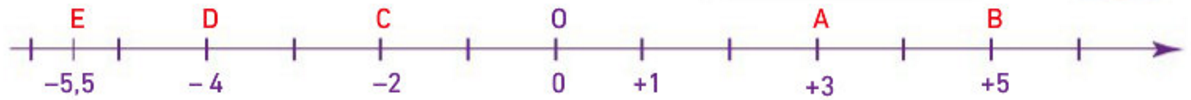
\includegraphics[scale=0.5]{img/droite2}		
	\end{center}

	\begin{multicols}{2}
		\begin{itemize}
		\item L'abscisse du point A est +3;
		\item L'abscisse du point B est +5;
		\item L'abscisse du point C est -2;
		\item L'abscisse du point D est -4.
		\item L'abscisse du point E est \num{-5.5};
		\item L'abscisse du point O est 0;
	\end{itemize}
	\end{multicols}
\end{myex}


\begin{mydefs}
	\begin{itemize}
		\item Un repère orthogonal est formé par deux droites graduées perpendiculaires et de même origine. La droite horizontale est l'\kw{axe des abscisses}, la verticale est l'\kw{axe des ordonnées}.
		
		\item Un point du plan est repéré par deux nombres relatifs, ses \kw{coordonnées}. Le premier nombre est son \kw{abscisse}, le second son \kw{ordonnée}. On note ces coordonnées $(abscisse \: ; \: ordonnée)$.
	\end{itemize}
\end{mydefs}


\begin{myexs}
	
		\begin{center}
			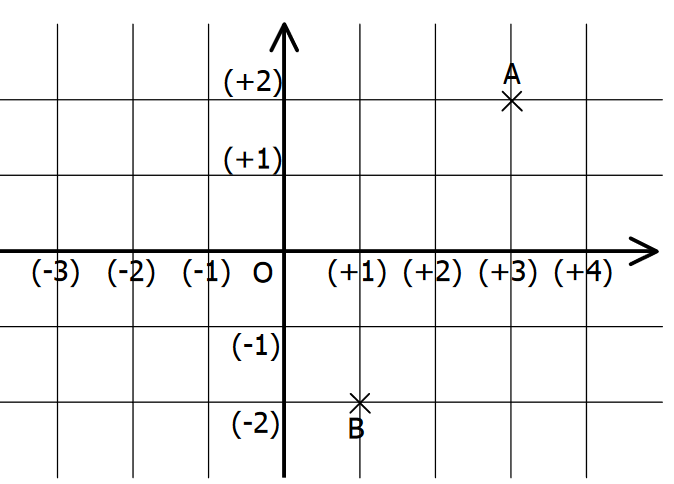
\includegraphics[scale=0.4]{repere}
		\end{center}
	

	\begin{itemize}
		\item L'abscisse du point $A$ est +3, son ordonnée est +2, ses coordonnées sont $(+3; +2)$.
		
		\item L'abscisse du point $B$ est +1, son ordonnée est -2, ses coordonnées sont $(+1; -2)$.
	\end{itemize}

\end{myexs}


\subsection{Comparaison}

 \newpage
 
\section{Addition et soustraction de deux nombres relatifs}

\begin{mymeth}
	Pour additionner ou soustraire deux fractions :
	
	\begin{enumerate}
		\item Je les écrit avec le \kw{même dénominateur};
		\item Je fais la \kw{somme des numérateurs};
		\item Je ne modifie pas le dénominateur;
	\end{enumerate}
\end{mymeth}

\begin{myexs}
	\begin{multicols}{3}
	
	
				\begin{eqnarray*}
					A &=& \frac{3}{5} + \frac{1}{5} \\
					A &=& \frac{3 + 1}{5}\\
					A &=& \frac{4}{5}\\
				\end{eqnarray*}
			
	
			\begin{eqnarray*}
				B &=& \frac{14}{3} - 2 \\
				B &=& \frac{14}{3} - \frac{2 \times 3}{3}\\
				B &=& \frac{14}{3} - \frac{6}{3}\\
				B &=& \frac{14 - 6}{3}\\				
				B &=& \frac{8}{3}\\
			\end{eqnarray*}
	
			\begin{eqnarray*}
				C &=& \frac{2}{3} + \frac{4}{9} \\
				C &=& \frac{2 \times 3}{3 \times 3} + \frac{4}{9}\\
				C &=& \frac{6}{9} + \frac{4}{9}\\
				C &=& \frac{6 + 4}{9}\\
				C &=& \frac{10}{9}\\
			\end{eqnarray*}
	
	\end{multicols}
\end{myexs}

\newpage

\section{Simplifications d'écriture}

\begin{mymeth}
	Pour alléger l'écriture d'une expression qui contient des nombres relatifs on peut :
	\begin{enumerate}
		\item \kw{Transformer les soustractions} en additions;
		\item Supprimer les \kw{symboles d'addition} et les \kw{parenthèses};
		\item Supprimer le \kw{signe du premier nombre} s'il est positif.
	\end{enumerate}
\end{mymeth}

\begin{myexs}
	
	On veut simplifier et calculer les expressions suivantes :
	\begin{eqnarray*}
		A &=& (+6) - (+5) + (-2) - (-4) + (+2)\\
		A &=& (+6) + (-5) + (-2) + (+4) + (+2)  \text{  \textit{(étape 1)}} \\
		A &=& +6  -5  -2  +4  +2 \text{  \textit{(étape 2)}}\\
		A &=& 6  -5  -2  +4  +2 \text{  \textit{(étape 3)}}\\
		A &=& 6 + 4 + 2 - 5 - 2 \\
		A &=& 12 - 7 \\
		A &=& 5 \\
	\end{eqnarray*}


	\begin{eqnarray*}
		B &=& (-4) + (-3) - (+8) - (-4) - (-7)\\
		B &=& (-4) + (-3) + (-8) + (+4) + (+7) \text{  \textit{(étape 1)}}\\
		B &=& -4  -3  -8  +4  +7 \text{  \textit{(étape 2)}}\\
		B &=& -15 + 11 \\
		B &=& -4 \\
	\end{eqnarray*}
\end{myexs}

\newpage

\begin{myrem}
	Toute expression peut s'écrire sous la forme d'une suite d'additions, et l'ordre des termes d'une addition ne change pas le résultat. On peut donc utiliser cette propriété pour regrouper les termes d'une expression de manière à faciliter les calculs.
\end{myrem}

\begin{myexs}
	\begin{multicols}{2}
		
	\begin{eqnarray*}
		C &=& - 7 + 4 - 8 + 7 - 4 \\
		C &=& (- 7 + 7) + (4 - 4) - 8  \\
		C &=& 0 + 0 - 8 \\
		C &=& -8
	\end{eqnarray*}


	\begin{eqnarray*}
		D &=& -2 + 4 - 8 + 5 + 6 \\
		D &=& (- 2 - 8) + (4 + 6) + 5 \\
		D &=& -10 + 10 + 5 \\
		D &=& 0 + 5 \\
		D &=& 5
	\end{eqnarray*}
	\end{multicols}
\end{myexs}



\end{document}

